\chapter{Descrizione classi}
\section{Modalspace}

Inizialmente ModalSpace \`e stata concepita per essere una classe base, dalla quale ereditasse ogni possibile scelta delle condizioni di bordo sulla parete del vaso. Facendo un rapido conto ci si accorge che comprendendo le condizioni di Dirichlet, Neumann e Robin su una sezione rettangolare arriviamo a 81 possibili combinazioni, una grande quanti\`a di codice da scrivere, che comprende casistiche molto simili fra loro se non identiche. Questo \`e stato il primo motivo che ci ha portato a scorporare il trattamento delle condizioni di bordo dalla classe ModalSpace, per poi includerlo in modo ottimale in Basis1DAbstract (classe che si occupa della gestione delle basi educate). Un secondo punto a favore di questa scelta riguarda la valutazione e la lettura delle basi modali. Se avessimo scelto di adottare l'ereditariet\`a in ModalSpace, ogni eventuale figlia avrebbe avuto un tipo di base differente e accedervi tramite la classe base ogni qual volta fosse necessario, non risultava essere efficiente. Dunque la struttura di ModalSpace \`e composta dalle valutazioni delle basi modali su un'opportuna griglia e i generatori di basi (oltre ai metodi di calcolo necessari), questo design attribuisce maggiore generalit\`a: ModalSpace \`e pronta ad utilizzare nuovi metodi in grado di generare una corretta base modale.

\subsection{Costruzione e setting}
ModalSpace conosce la geometria della sezione (Ly, Lz) e sicuramente deve conoscere il grado di accuratezza desiderato dall'utente, ovvero il numero di modi da utilizzare (mtot). 
Un altro punto fondamentale del costruttore generico \`e senz'altro la regola di quadratura da utilizzare sulla slice. Si noti che le basi utilizzate necessitano regole di quadratura di alto ordine e il grado di esattezza \`e strettamente legato al numero di modi. Questo legame \`e evidente se si pensa che maggiore \`e il modo, maggiore sar\`a la frequenza della base modale e conseguentemente si avr\`a bisogno di una fitta successione di nodi di quadratura. Su una sezione quadrata una buona approssimazione dei nodi necessari su ciascun lato \`e $\sqrt{mtot}$. Il risultato non \`e valido nel caso di sezioni molto asimmetriche, infatti rettangoli molto allungati in una direzione avranno bisogno di pi\`u nodi lungo la direzione maggiore e meno sull'altra. Come esempio si osservi la seguente tabella dove sono riportati i check dei valori di normalit\`a di una base, fissata la regola di quadratura al variare della dimensione $L_y$.

\begin{center}
\begin{tabular}{|c|c|c|c|c|}
\hline
Lx&Ly & Max(p,q) &  $\parallel err32 \parallel_{L_{\inf}}$ &  $\parallel err64 \parallel_{L_{\inf}}$ \\
\hline
1.0&2.0 & 12 & 1.85391e-9 & 9.54883e-14 \\
\hline
1.0&4.0 & 16 & 8.7809e-4 & 1.51567e-13 \\
\hline
1.0&8.0 & 23 & 7.87756 & 2.70061e-13 \\
\hline
1.0&16.0 & 33 & 54.7566 & 7.91844e-6 \\
\hline
1.0&32.0 & 50 & 185.541 & 32.7153 \\
\hline
\end{tabular}
\end{center}


Una volta creato l'oggetto \texttt{ModalSpace} bisogna eseguire alcuni set importanti. Per prima cosa dobbiamo impostare i generatori di base lungo le direzioni trasversali. Nel caso di basi educate questa operazione viene eseguita assieme all'imposizione delle condizioni di parete tramite i metodi pubblici:
\begin{itemize}
\item \texttt{void AddSliceBCY(const string left, const string right, const Real mu = 1, const Real Chi =1)};
\item \texttt{void AddSliceBCZ(const string left, const string right, const Real mu = 1, const Real Chi =1)}
\end{itemize}

\begin{lstlisting}[style = general]
void ModalSpace::
AddSliceBCY (const string& left, const string& right, const Real& mu, const Real& chi)
{
	M_genbasisY = Basis1DFactory::istance().createObject(left+right;)
	M_genbasisY->setL(M_Ly);
	M_genbasisY->setMu(M_mu);
	M_genbasisY->setChi(chi)
	
	return;
}
\end{lstlisting}
 Nel caso si desideri aggiungere nuove tipologie di basi, queste dovranno essere ereditate dall'oggetto \texttt{Basis1DAbstract}, il quale conferisce una struttura generale al generatore di basi, osservando le ipotesi descritte nella sezione \referenza{sec: ipotesi}.
 
 \begin{equation}
\textcolor{red}{Aprire il discorso della factory, meglio farlo insieme} 
 \end{equation}

Infine si conlude il seting della classe ModalSpace tramite la funzione membro pubblica EvaluateBasis(), che chiama le funzioni adibite a riempire le strutture dati, che mostriamo nella seguente sezione.

\begin{lstlisting}[style = general]
boost::shared_ptr<ModalSpace> MB (new ModalSpace(Ly,Lz,mtot,quadY,quadZ));
MB ->AddSliceBCY("dir","dir");
MB ->AddSliceBCZ("rob","rob",1.,3.);
MB ->EvaluateBasis();
\end{lstlisting}

\subsubsection{Strutture dati}
Diamo un breve descrizione delle strutture dati possedute dalla classe ModalSpace. Per prima cosa per\`o, occupiamoci di un aspetto fondamentale. Le basi modali sono determinate sull'intervallo di riferimento, per non incorrere in errori fra dominio reale e riferimento,  utilizzeremo la seguente notazione:
\begin{equation}
\label{eq: notazione}
\begin{array}{l l l}
\hat{\varphi}_j(\hat{y},\hat{z}) = \hat{\eta}_j(\hat{y}) \hat{\xi}_j(\hat{z}) & \hat{y} \in [0,1] & \hat{z} \in [0,1] 
\\
\\
\int_0^1 \hat{\eta}^2_j\,d\hat{y} = 1 & \int_0^1 \hat{\xi}^2_j\,d\hat{z} = 1
\end{array}
\end{equation}
Dove $\hat{\varphi_j}$ \`e la base modale ortonormale sul dominio di riferimento, risultato del prodotto delle basi ottenute tramite i generatori di basi.
Vediamo ora come gestire il passaggio dalle basi definite sul riferimento a quelle invece sul dominio reale. L'ortogonalit\`a si conserva facilmente, ma lo stesso discorso non vale per la normalizzazione. Verifichiamo che un semplice cambio di coordinate non conserva la normalizzazione:

\begin{equation}
\label{eq: trasformazione}
\begin{array}{l l }
\int_0^{L_y}\int_0^{L_z} \varphi_j(y,z)^2 \,dydz 
\\
\\
= \int_0^{L_y} \eta_j(y)^2 \,dy\int_0^{L_z} \xi_j(z)^2 \,dz 
\\
\\
= \int_0^{1} \eta_j(L_y\hat{y})^2 L_y\,d\hat{y} \int_0^{1} \xi_j(L_z\hat{z})^2 L_z\,d\hat{z} 
\\
\\
 = L_yL_z\int_0^{1} \hat{\eta}_j(\hat{y})^2 \,d\hat{y} \int_0^{1} \hat{\xi}_j(\hat{z})^2 \,d\hat{z} & \neq  1  
\end{array}
\end{equation}

Da questi semplici passaggi deduciamo che per essere mantenere la normalizzazione, la base che stiamo cercando avr\`a la seguente forma:
\begin{equation}
\label{eq: base sul dominio corrente}
\varphi_j(y,z) = (L_yL_z)^{-\frac{1}{2}}\hat{\eta}_j(yL_y^{-1})\hat{\xi}_j(zL_z^{-1})
\end{equation}
In conclusione, nei conti che verranno proposti si faccia sempre riferimento all'equazione \referenzaeq{eq: base sul dominio corrente}.

Riconosciamo cinque strutture dati fondamentali per la classe \texttt{ModalSpace}:

\begin{itemize}

\item \texttt{EigenContainer M\_eigenvalues}, contiene le sottofrequenze e gli indici corrispondenti, viene prodotta in fase di setting dello spazio modale tramite la funzione membro \texttt{EigensProvider()}, chiamata da \texttt{EvaluateBasis()}. Il tipo \`e un \texttt{vector$<$EigenMap$>$} dove:
 
\begin{lstlisting}[style = general]
struct EigenMap
{
	Real wp;	//subfrequency y
	Real wq;	//subfrequency z
	UInt p;
	UInt q;
	
	static EigenMap make_eigenmap(const Real& _wp,const Real& _wq,const UInt& _p,const UInt& _q)
	{
		EigenMap a;
		a.wp = _wp;
		a.wq = _wq;
		a.p = _p;
		a.q = _q;
		return a;	
	}
};
\end{lstlisting}
L'ordinamento gerarchico degli autovalori e la corrispondenza delle sottofrequenze con i sottoindici \`e fondamentale, approfondiremo in seguito il metodo \texttt{EigensProvider()}.

\item \textbf{MBMatrix\_type M\_phiy}, \`e un \texttt{vector$<$vector$<$Real$>$ $>$} che raccoglie la valutazione di $\hat{\eta}_j(\hat{y})$ $\forall j$ e per ogni nodo di quadratura lungo $\hat{y}\in[0,1]$.

\item \textbf{MBMatrix\_type M\_phiz}, \`e un \texttt{vector$<$vector$<$Real$>$ $>$} che raccoglie la valutazione di $\hat{\xi}_j(\hat{y})$ $\forall j$ e per ogni nodo di quadratura lungo $\hat{z}\in[0,1]$.

\item \textbf{MBMatrix\_type M\_dphiy}, \`e un \texttt{vector$<$vector$<$Real$>$ $>$} che raccoglie la valutazione di $\frac{\partial\hat{\eta}_j}{\partial 	\hat{y}}$ $\forall j$ e per ogni nodo di quadratura lungo $\hat{y}\in[0,1]$.

\item \textbf{MBMatrix\_type M\_dphiz}, \`e un \texttt{vector$<$vector$<$Real$>$ $>$} che raccoglie la valutazione di $\frac{\partial\hat{\xi}_j}{\partial 	\hat{z}}$ $\forall j$ e per ogni nodo di quadratura lungo $\hat{z}\in[0,1]$.

\end{itemize}


\subsection{Metodi di calcolo}
Approfondiamo ora i metodi che si occupano di calcolare i coefficienti della matrice di sistema.

\begin{itemize}
\item \texttt{Real Compute\_PhiPhi(const UInt\& j, const UInt\& k)}

 $\int_{\gamma_x}\varphi_j(y,z)\varphi_k(y,x) \,dydz$

\item \texttt{Real Compute\_DyPhiPhi(const UInt\& j,const UInt\& k)} 

$\int_{\gamma_x} \partial_y \varphi_j(y,z)\varphi_k(y,x) \,dydz$

\item \texttt{Real Compute\_DzPhiPhi(const UInt\& j,const UInt\& k)} 

$\int_{\gamma_x} \partial_z \varphi_j(y,z)\varphi_k(y,x) \,dydz$

\item \texttt{Real Compute\_DyPhiDyPhi(const UInt\& j,const UInt\& k)} 

$\int_{\gamma_x} \partial_y \varphi_j(y,z)\partial_y\varphi_k(y,x) \,dydz$

\item \texttt{Real Compute\_DzPhiDzPhi(const UInt\& j,const UInt\& k)} 

$\int_{\gamma_x} \partial_z \varphi_j(y,z)\partial_z\varphi_k(y,x) \,dydz$

\item \texttt{Real Compute\_Phi(const UInt\& k)} 

$\int_{\gamma_x} \varphi_k(y,x) \,dydz$

\item \texttt{vector$<$Real$>$ FourierCoefficients (const function\_Type\& g) const},

data una funzione indipendente da $x$ questo metodo restituisce i coefficienti di Fourier (in numero pari ad \texttt{M\_mtot}) rispetto alla base modale scelta.

\item \texttt{Real Coeff\_fk (	const Real\& x,const function\_Type\& f,const UInt\& k ) const},

restituisce il $k$-esimo coefficiente di Fourier di una generica funzione 3D valutato nel punto $x$, rispetto alla base modale.
\end{itemize}

Date le premesse risulta ora semplice risolvere gli integrali scritti qui sopra, vediamo ad esempio che aspetto ha \texttt{Compute\_PhiPhi()}:


\begin{lstlisting}[style = general]
Real ModalSpace::
Compute_PhiPhi(const UInt& j, const UInt& k) const
{
	Real coeff_y = 0.0;
	Real coeff_z = 0.0;
	UInt p_j = M_eigenvalues[j].p-1;
	UInt p_k = M_eigenvalues[k].p-1;
	UInt q_j = M_eigenvalues[j].q-1;
	UInt q_k = M_eigenvalues[k].q-1;
	
	Real normy = 1.0 / sqrt(M_Ly);
	Real normz = 1.0 / sqrt(M_Lz);
	
	for(UInt n = 0; n < M_quadruleY->nbQuadPt();++n)
	{
		coeff_y +=	M_phiy[p_j][n] * normy *	
							M_phiy[p_k][n] * normy *
							M_Ly * M_quadruleY->weight(n);
	}
	
		for(UInt n = 0; n < M_quadruleZ->nbQuadPt();++n)
	{
		coeff_z +=	M_phiz[q_j][n] * normz *	
							M_phiz[q_k][n] * normz *
							M_Lz * M_quadruleZ->weight(n);
	}
	
	return coeff_y*coeff_z;
}
\end{lstlisting}
 
 Gli ultimi due metodi citati sono indispendabili ed il loro impiego sar\`a noto una volta che tratteremo la classe \texttt{HiModAssembler}.
 
 \subsection{\texttt{EigensProvider()}}
 Abbiamo deciso di dedicare una sezione solamente a questo metodo, poich\'e la ricerca degli autovalori occupa un ruolo fondamentale nella struttura del codice.
 Il metodo viene chiamato da \texttt{EvaluateBasis()} dunque dopo che sono stati settati i generatori di basi. La funzione deve preoccuparsi di definire la struttura dati \texttt{M\_eigenvalues}, tuttavia il procedimento non \`e scontato. 
 Per comprendere le difficolt\`a occorre ragionare sulla struttura del problema. Separando le variabili della slice 2D si sono ottenuti due problemi agli autovalori 1D (sezione \referenza{sec: ipotesi}). Ognuno di questi genera una successione ordinata crescente di autovalori, determinata dalla risoluzione del problema agli autovalori, che nel caso di basi educate si traduce nella ricerca degli zeri di una data funzione non lineare. Definiamo la successione di autovalori in $y$ con $\{K_y\}_p$ e quella in $z$ con $\{K_z\}_q$. Le precedenti successioni definiscono univocamente la successione degli autovalori del problema di partenza 2D e sono in relazione con essa nel seguente modo:

\begin{equation}
\label{eq: autovalori}
 \lambda_j = (K_y^p)^2 + (K_z^q)^2
\end{equation} 

Anche $\{\lambda\}_j$ \`e una successione crescente di autovalori, ma il suo ordinamento, dato quello dei sottoautovalori, non \`e immediato. Due sono le difficolt\`a che si presentano:
\begin{itemize}
\item[1.] Ogni sottoautovalore \`e il risultato di una ricerca di zeri di una funzione non lineare.
\item[2.] L'utente stabilisce il numero massimo di modi sul problema 2D e non sui sotto-problemi 1D.
\end{itemize}

Le due problematiche sono strettamente legate, difatti non siamo interessati a cercare pi\`u sottoautovalori del necessario. Si poteva partire calcolando ad esempio 10 sottoautovalori in $y$ e altrettanti in $z$, ordinare la succession 2D e procedere eventualmente nella ricerca. Questo metodo tuttavia presenta due difetti: \`e poco efficiente ed inoltre pu\`o cadere in errore. Infatti l'algoritmo si dovrebbe fermare una volta raggiunti un numero di autovalori 2D pari ad \texttt{M\_mtot}, ma cos\`i facendo nessuno ci assicura che nel gruppo successivo di 10 autovalori non vi sia almeno uno minore dell'ultimo autovalore calcolato.

La soluzione \`e stata quella di procedere un passo alla volta, con l'accortezza di salvare i sotto-autovalori ancora non utlizzati. Per fare questo il metodo di ricerca degli zeri (\texttt{Next()} che approfondiremo nella sezione \texttt{Basis1DAbstract}) fornisce progressivamente uno zero alla volta. Infine abbiamo analizzato il seguente albero delle scelte:


\begin{lstlisting}[style = general,frame = top]
Ky_1 = NextY();
Kz_1 = Nextz();
-> La prima coppia viene sempre inserita nella mappa
-> Cerco Ky_2 e Kz_2 nella mappa o nel registro
		if(trovati) -> li assegno a Ky_2 Kz_2;
		else		Ky_2 = NextY();
						Kz_2 = Nextz();
-> Inserisco nella mappa la coppia di sottoautovalori minore
-> Registro i sottoautovalori non inseriti
\end{lstlisting}
\begin{tikzpicture}[stack/.style={
  rectangle split, rectangle split parts=5, draw, anchor=center},
  myarrow/.style={single arrow, draw=none}]

\node [stack] (prima)  {\nodepart{two}
\nodepart{three}\nodepart{four}
\nodepart{five}$Ky^{(1)},Kz^{(1)}$};

\node [stack,right=of prima] (seconda) {\nodepart{two}
  \nodepart{three}\nodepart{four}$Ky^{(1)},Kz^{(2)}$
  \nodepart{five}$Ky^{(2)},Kz^{(1)}$};

\node [stack,right=of seconda] (terza) {{\nodepart{two}
\nodepart{three}\nodepart{four}$Ky^{(2)},Kz^{(1)}$
\nodepart{five}$Ky^{(1)},Kz^{(1)}$};

\node [stack,right=of terza] (quarta) {\nodepart{two}
  \nodepart{three}\nodepart{four}
  \nodepart{five}$Ky^{(1)},Kz^{(2)}$};
  
\node [above=of prima,anchor=north,align=left] {Eigenvalues};
\node [above=of seconda,anchor=north,align=left] {Tmp};

\node [myarrow,draw,anchor=west] at ($(seconda.east)+(2.5pt,0)$) {\phantom{te}} ;

%\node [myarrow,draw,anchor=west] at ($(mid.east)+(2.5pt,0)$) %{\phantom{te}} ;
\draw [red,ultra thick,->] ($(seconda.west)+(-0.1,-1.0)$) -- ($(prima.east)+(0.1,-0.4)$);
\draw [red,thick] ($(seconda.south)+(-1.4,-0.2)$)--($(seconda.south)+(1.4,0.8)$);
\draw [red,thick] ($(seconda.south)+(-1.4,0.8)$)--($(seconda.south)+(1.4,-0.2)$);

 % {instruction 0;\\ instruction 1;\\$\ldots$\\instruction $n$;};
\end{tikzpicture}
%\begin{tikzpicture}
%[scale=1.5]
%\tikzstyle{every node}=[draw,shape=rectangle];
%\path (5,0)   node (v1) {$Ky^{(1)},Kz^{(1)}$};
%\path (3,-1) node (v2) {$Ky^{(2)},Kz^{(1)}$};
%\draw (v1) -- (v2);
%\end{tikzpicture}


\begin{lstlisting}[style = general,frame = top]
-> Cerco Ky_3 e Kz_2 nella mappa o nel registro
		if(trovati) -> li assegno a Ky_3 Kz_2;
		else		Ky_2 = NextY();
						Kz_2 = Nextz();
-> Inserisco nella mappa la coppia di sottoautovalori minore rispetto anche a quelli nel registro
-> Registro i sottoautovalori non inseriti
\end{lstlisting}
\begin{tikzpicture}[stack/.style={
  rectangle split, rectangle split parts=5, draw, anchor=center},
  myarrow/.style={single arrow, draw=none}]

\node [stack] (prima) {{\nodepart{two}
\nodepart{three}\nodepart{four}$Ky^{(2)},Kz^{(1)}$
\nodepart{five}$Ky^{(1)},Kz^{(1)}$};

\node [stack,right=of prima] (seconda) {\nodepart{two}
  \nodepart{three}$Ky^{(2)},Kz^{(2)}$\nodepart{four}$Ky^{(3)},Kz^{(1)}$
  \nodepart{five}$Ky^{(1)},Kz^{(2)}$};
  
  \node [stack,right=of seconda] (terza)  {\nodepart{two}
\nodepart{three}$Ky^{(1)},Kz^{(2)}$\nodepart{four}$Ky^{(2)},Kz^{(1)}$
\nodepart{five}$Ky^{(1)},Kz^{(1)}$};

\node [stack,right=of terza] (quarta) {\nodepart{two}
  \nodepart{three}\nodepart{four}$Ky^{(2)},Kz^{(2)}$
  \nodepart{five}$Ky^{(3)},Kz^{(1)}$};
  
\node [above=of prima,anchor=north,align=left] {Eigenvalues};
\node [above=of seconda,anchor=north,align=left] {Tmp};

\node [myarrow,draw,anchor=west] at ($(seconda.east)+(2.5pt,0)$) {\phantom{te}} ;

%\node [myarrow,draw,anchor=west] at ($(mid.east)+(2.5pt,0)$) %{\phantom{te}} ;
%\node [draw,rectangle,align=left,right=of ini,label=above:%{Computer Program}] (mid)
 % {instruction 0;\\ instruction 1;\\$\ldots$\\instruction $n$;};
\end{tikzpicture}
%\begin{tikzpicture}
%[scale=1.5]
%\tikzstyle{every node}=[draw,shape=rectangle];
%\path (5,0)   node (v1) {$Ky^{(1)},Kz^{(1)}$};
%\path (3,-1) node (v2) {$Ky^{(2)},Kz^{(1)}$};
%\path (7,-1) node (v3) {$Ky^{(1)},Kz^{(2)}$};
%\draw (v1) -- (v2)
%(v1) -- (v3);
%\end{tikzpicture}


\begin{lstlisting}[style = general,frame=top]
-> inserimento di copie evitato per unicita' degli oggetti nella struttura scelta
(Ky_2,Kz_2) già esistente non viene inserito nella mappa
\end{lstlisting}
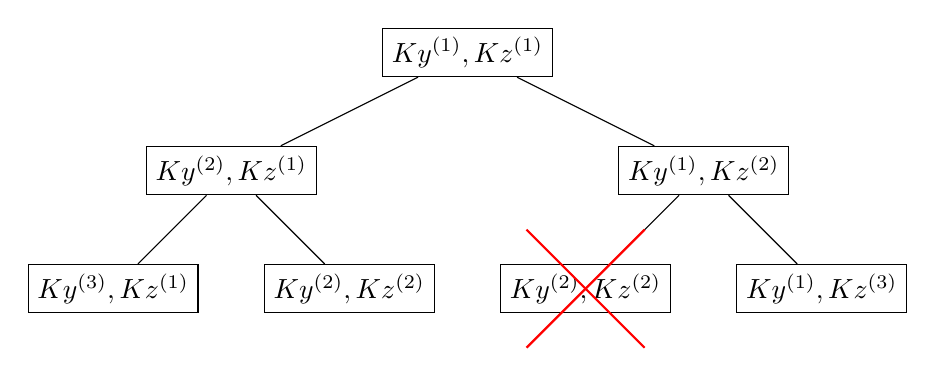
\begin{tikzpicture}
[scale=1.5]
\tikzstyle{every node}=[draw,shape=rectangle];
\path (5,0)   node (v1) {$Ky^{(1)},Kz^{(1)}$};
\path (3,-1) node (v2) {$Ky^{(2)},Kz^{(1)}$};
\path (7,-1) node (v3) {$Ky^{(1)},Kz^{(2)}$};
\path (2,-2) node (v4) {$Ky^{(3)},Kz^{(1)}$};
\path (4,-2) node (v5) {$Ky^{(2)},Kz^{(2)}$};
\path (6,-2) node (v6) {$Ky^{(2)},Kz^{(2)}$};
\path (8,-2) node (v7) {$Ky^{(1)},Kz^{(3)}$};
\draw (v1) -- (v2)
(v1) -- (v3)
(v2) -- (v4)
(v2) -- (v5)
(v3) -- (v6)
(v3) -- (v7);
\draw [thick,red, -] (5.5,-1.5)--(6.5,-2.5);
\draw [thick,red, -] (6.5,-1.5)--(5.5,-2.5);
\end{tikzpicture}



 \section{Basis1dAbstract}

Questa classe si occupa di definire dei generatori di base, ovvero gli oggetti puntati nella classe \texttt{ModalSpace} dai membri \texttt{M\_genbasisY} e \texttt{M\_genbasisZ}. Ereditando la struttura generale basata solamente sulle ipotesi\referenza{sec: ipotesi}, abbiamo implementato delle classi derivate seguendo la teoria delle Educated Basis (E.B.). La struttura polimorfica sembra bene adattarsi alle possibili evoluzione future del problema, poich\'e diverse teorie sulla scelta delle basi sono tutt'ora in fase di sviluppo.
 
\subsubsection{I metodi}

La classe base \`e astratta, da essa derivano nove classi figlie, le quali corrispondono alle possibili combinazioni di condizioni di bordo omogenee di un problema 1D. Ogni classe figlia eredita pubblicamente da \texttt{Basis1DAbstract} ed implementa in modo proprio i seguenti metodi:

\begin{itemize}
\item \texttt{Real Next()} 
\item \texttt{void EvaluateBasis()}
\item \texttt{Real EvalSinglePoint()}
\end{itemize}

I primi due metodi sono usati nella fase di set dell'oggetto modalspace, mentre l'ultimo \`e un utilit\`a della quale ne vedremo l'applicazione nella fase di export posseduta da HiModAssembler. 

Il membro principale di ogni classe figlia \`e \texttt{M\_ptrfunctor}. 
L'unica eccezione \`e il caso Dirichlet su entrambe i bordi, nell'osservazione in \referenza{sec: educated basis} abbiamo sottolineato la trivialit\`a di questo caso, che non necessita la definizione del funtore.
L'oggetto puntato da questo shared\_pointer  \`e un \texttt{EducatedBasisFunctor}. Abbiamo scelto di costruire un sistema di classe base e derivate ausiliario, simile strutturalmente a \texttt{Basis1DAbstract}: la classe base \`e costituita da \texttt{EducatedBasisFunctorAbastract} e vi \`e una classe figlia per ogni possibile combinazione di condizioni di bordo di un problema 1D (dunque nove come le classi figlie di \texttt{Basis1DAbstract}), per ognuna di esse \`e implementato solamente l'operatore \texttt{()}. Ogni funzione ricavata dalla risoluzione dei problemi agli autovalori, \`e contenuta in quesa gerarchia di classi ausiliarie. Il costruttore \`e comune a tutte le classi figlie, ed \`e quindi definito solamente nella classe base, esso si occupa di settare in maniera corretta i parametri riferiti alle condizioni di bordo applicate ($\mu$ e $\chi$). 


I restanti membri hanno l'utilit\`a di memorizzare quale autovalore \`e stato calcolato per ultimo, in questo modo il metodo \texttt{Next()} \`e in grado di procedere al calcolo progressivo di tutti gli autovalori desiderati, senza tornare sui suoi passi. Per comprendere meglio la distribuzione degli autovalori, mostriamo nella seguente figura la forma della funzione non lineare nel caso Robin-Robin.

\begin{equation}
FIGURA
\end{equation}

Abbiamo visto che \texttt{ModalSpace} possiede il metodo \texttt{EvaluateBasis()}, in realt\`a questa funzione chiama separatamente i metodi omonimi, di propriet\`a dei due generatori di basi, poich\'e sono loro a conoscere la forma delle funzioni di base. L'implementazione di \texttt{EvaluateBasis()} \`e semplice, l'obbiettivo \`e il completamento di una delle strutture dati matriciali possedute da \texttt{ModalSpace}. In particolare il generatore \texttt{M\_genbasisY} si occuper\`a di \texttt{M\_phiy} e \texttt{M\_dphiy}, mentre \texttt{M\_genbasisZ} completer\`a le restanti strutture.
Facendo riferimento alla forma generica delle basi modali \referenzaeq{eq: 1sottoproblema}, \`e chiaro che il compito di \texttt{EvaluateBasis()} \`e di calcolare i coefficienti A e B in modo tale che le basi rispettino le condizioni di bordo e risultino normali (ricordiamo che l'ortogonalit\`a \`e garantita dalla teoria).

La registrazione delle valutazioni della base modale nei nodi di quadratura \`e un'operazione necessaria al fine di velocizzare le operazioni di integrazione. Tuttavia come procediamo se siamo interessati a valori delle basi su una griglia pi\`u fitta di quella di quadratura? Per risolvere questo problema \`e stato scritto il metodo \texttt{EvalSinglePoint()} che dato un sotto autovalore e la coordinata, restituisce la valutazione della base modale in quel dato punto. Questa funzione si \`e resa necessaria dal momento che in fase di export desideravamo interpolare la funzione su una griglia con pi\`u nodi rispetto alla quadratura.

\begin{figure}[!htbp]
        \centering%
          {\label{fig: slice9}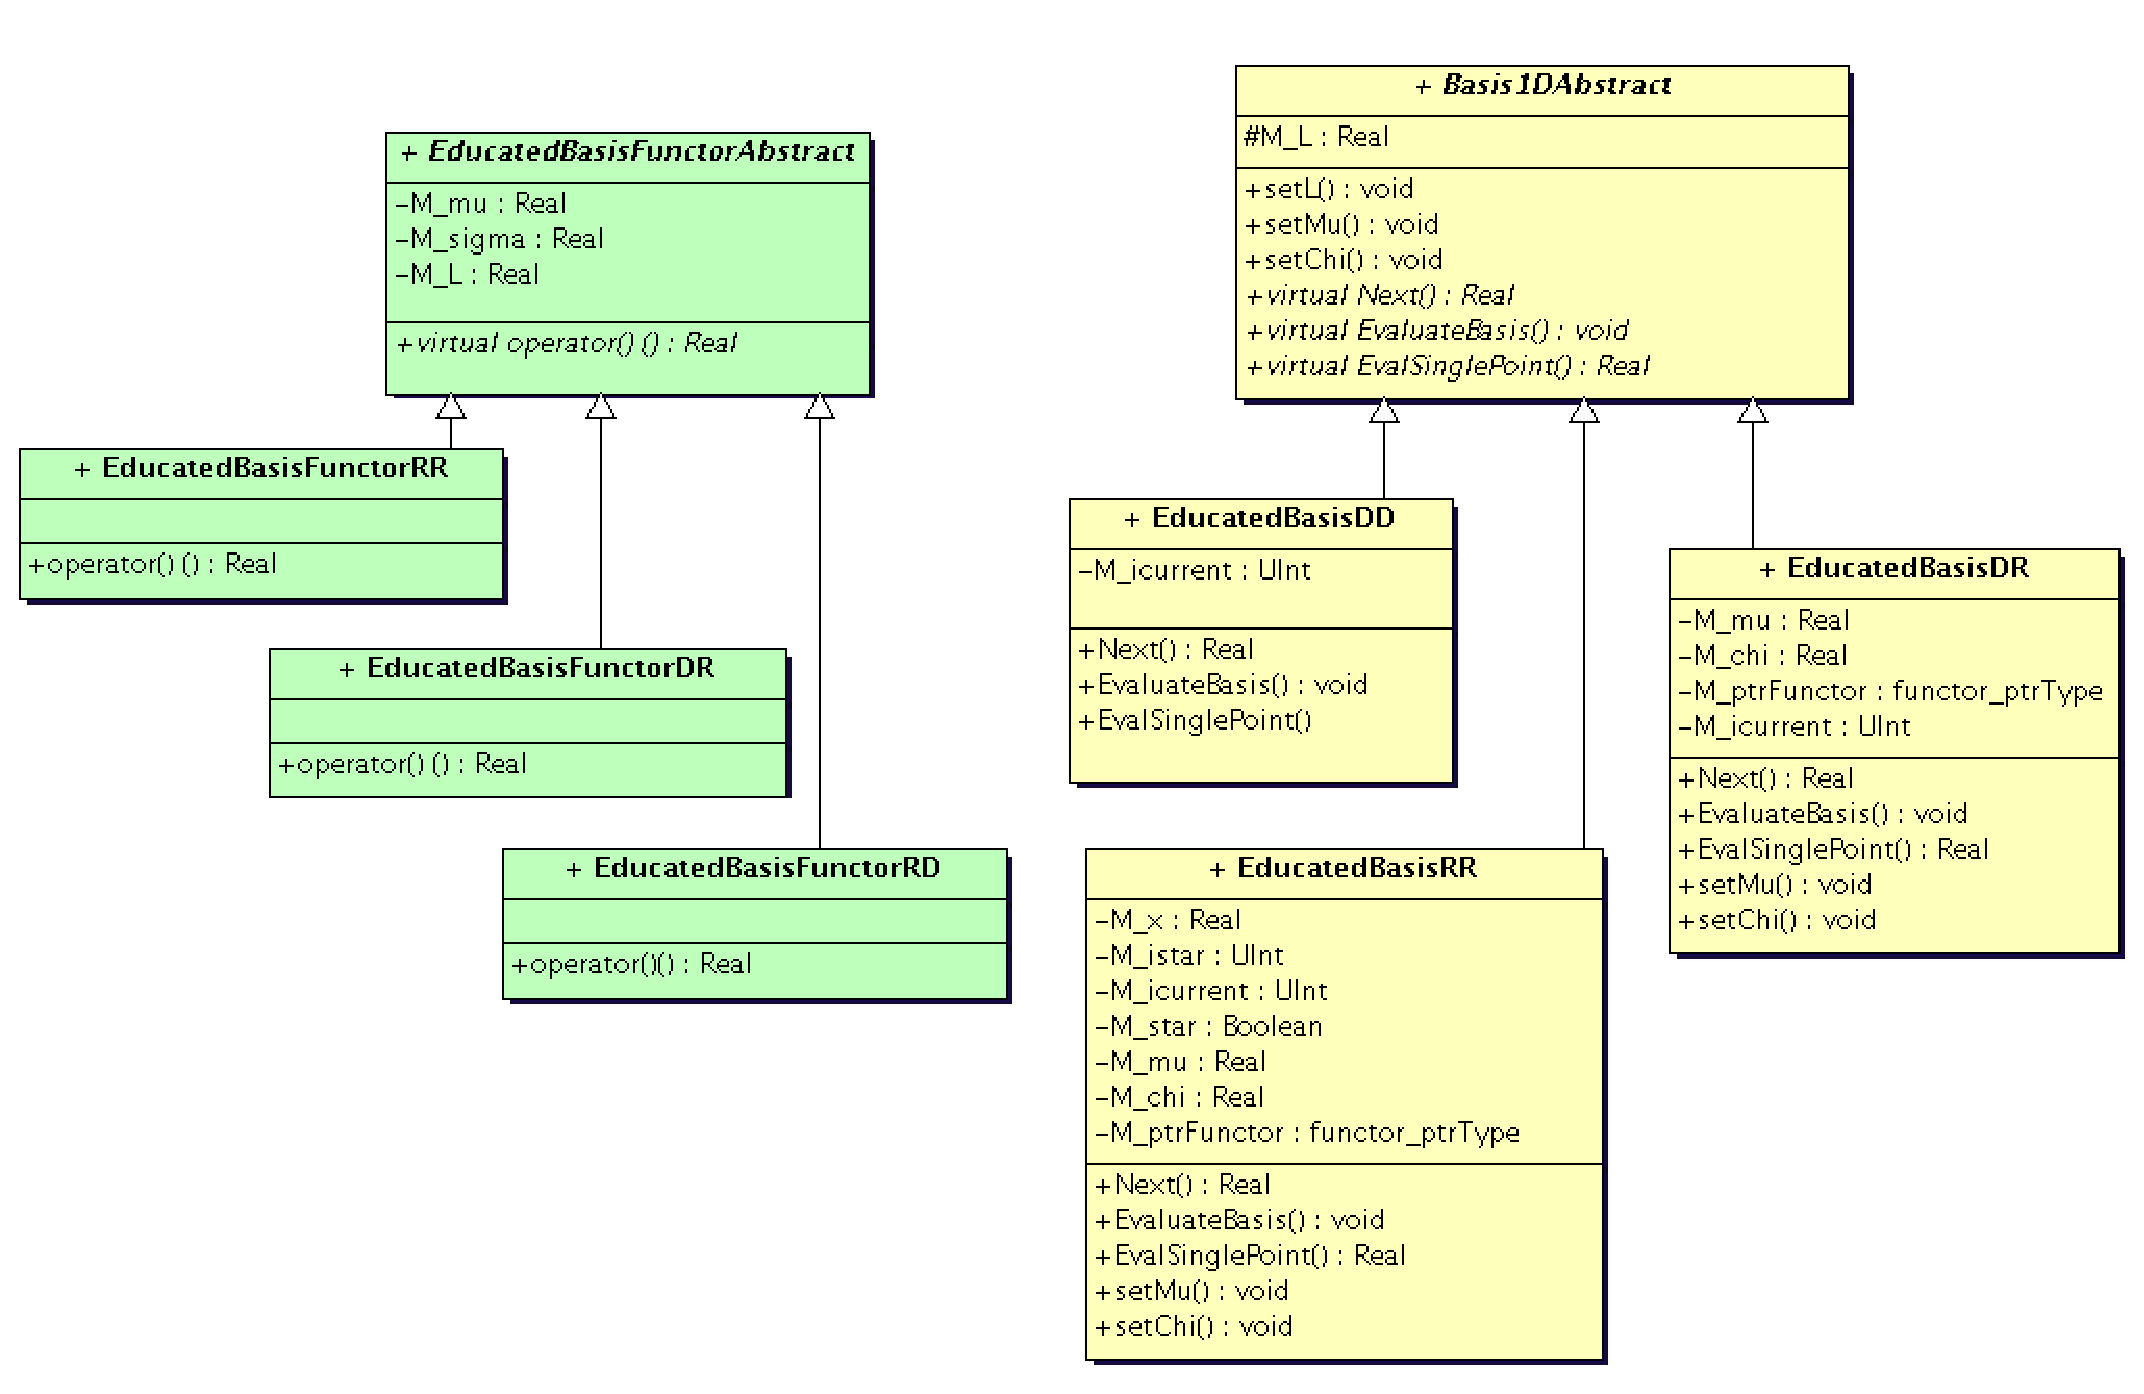
\includegraphics[scale=0.33]{UML/Basis1DAbstract.eps}}\qquad
        \caption{Classi Basis1DAbstract e EducatedBasisFunctor}
        \label{fig: UMLBasis}
\end{figure}

\section{HiModAssembler}
 
 In questa classe viene gestita la fase di assemblaggio del problema e quella di export. Abbiamo cercato di seguire la linea della classe FESpace, infatti \texttt{HiModAssembler} \`e templetizzata sugli stessi argomenti. Oltre a mantenere una struttura di base coerente con lo spazio agli elementi finiti, la scelta di templetizzare le matrici e i vettori, manipolati da tale classe, prevede una possibile implementazione futura di strutture algebriche pi\`u adatte al metodo di riduzione gerarchica. Ricordiamo infatti che la struttura della matrice di sistema \`e ben nota \figref{fig:pattern} , formata da un numero di blocchi pari ad $\texttt{M\_mtot}^2$, ognuno dei quali di dimensione pari al quadrato dei gradi di libert\`a FEM spesi lungo la fibra di supporto.
 

 
 Viene templetizzata anche la mesh, ma questo parametro si riferisce discretizzazione della fibra di supporto, dunque siamo vincolati a trattarlo in questo modo.
 Momentanemante il codice funziona solamente con elementi del tipo EpetraStructured, tuttavia occorrerebbe ripensare attentamente questa parte, soprattutto in visione di una possibile parallelizzazione.
Un codice HiMod ottimizzato dovr\`a possedere delle proprie strutture, adeguate alla conformazione della matrice di sistema.

 \begin{lstlisting}[style = general]
 template<typename mesh_type,typename matrix_type,typename vector_type>
 class HiModAssembler
 {
	... 
 };
 \end{lstlisting}
 
\subsubsection{I membri}
La classe HiModAssembler posside tre membri privati:

\begin{itemize}
\item \texttt{modalbasis\_ptrType M\_modalbasis
\item \texttt{fespace\_ptrType M\_fespace
\item \texttt{etfespace\_ptrType M\_etfespace}}}
\end{itemize}

Nota la teoria era chiaro che la classe dovesse possedere lo spazio modale 2D e lo spazio elementi finiti 1D.
Il restante oggetto esiste per una scelta di programmazione. Infatti abbiamo deciso di ricorrere all'utilizzo del pacchetto \texttt{ETA}, piuttosto che del \texttt{GeneralAssembler}. Due sono le motivazioni che hanno condotto a questa scelta:
\begin{itemize}
\item[1.] Semplicit\`a di scrittura della forma variazionale.
\item[2.] Possibilit\`a di scrivere pi\`u parti di forma variazionale.
\end{itemize}

Entrambe le motivazioni sono legate in realt\`a a possibili future estensioni del codice. Se pensiamo al problema generalizzato ad una qualunque sezione 2D, siamo costretti ad adottare una mappa che leghi lo spazio reale e lo spazio di riferimento (dove viene risolto il problema). I conti mostrano che alla forma variazionale si aggiungono numerosi casi non gestiti dal pacchetto \texttt{GeneralAssembler}.

L'utilizzo del modulo \texttt{ETA} \`e tuttavia nascosto all'utente, il costruttore si occupa di inizializzare \texttt{M\_etfespace} ricavando le informazioni necessarie da \texttt{M\_fespace}.

\begin{lstlisting}[style=general]
 template<typename mesh_type,typename matrix_type,typename vector_type>
 HiModAssembler<mesh_type, matrix_type,vector_type>::
 HiModAssembler(	const fespace_ptrType& fespace,
 									const modalbasis_ptrType& modalbasis,
 									commPtr_Type& Comm):
 		M_Modalbasis	( modalbasis),
 		M_etfespace 	( new etfespace_type (fespace->mesh(),
 																 &(fespace->refFE()),
 																 &(fespace->fe().geoMap()),
 																 Comm))
		M_fespace		( fespace)
{} 																 
 																
\end{lstlisting}

\subsection{I metodi}
Proponiamo di seguito una descrizione dei vari metodi disponibili nella classe \texttt{HiModAssembler}. La classe \`e ampia, tuttavia comprende tre sezioni ben distinte: assemblaggio, analisi e export.
\subsubsection{Assemblaggio}
\begin{lstlisting}[style=general, frame = top]

void AddADRProblem	( const matrix_ptrType& systemMatrix,
											const Real& mu, 
											const TreDvector_type& beta, 
											const Real& sigma)
\end{lstlisting}
Si occupa dell'assemblaggio della matrice di sistema. I coefficienti sono considerati costanti (ipotesi \referenza{sec: ipotesi}), l'estensione a coefficienti non costanti comporta cambiamenti anche nella classe \texttt{ModalSpace}, tali modifiche non sono state apportate perch\`e esuli dai nostri obbiettivi progettuali. Si \`e ragionato su una possibile implementazione che segue la linea generale proposta negli articoli (citazione perotto).
Le fasi di assemblaggio sono semplici: la matrice di sistema viene percorsa a blocchi e per ognuno di essi il computo dei valori avviene tramite il metodo \texttt{integrate} del pacchetto \texttt{ETA}. Difatti ogni blocco corrisponde al problema 1D che accoppia la frequenza \texttt{j} e \texttt{k}.

\begin{lstlisting}[style = general, frame = top]

void interpolate	( const function_Type& f,
										const vector_ptrType& f_interpolated)
\end{lstlisting}
Data una generica funzione spaziale, questo metodo si occupa di calcolare, per ogni punto della griglia 1D, tutte le componenti di Fourier rispetto alle basi modali. Il risultato viene salvato nel vettore strutturato passato negli argomenti. \`E in questo punto che ricopre un ruolo fondamentale il metodo \texttt{Coeff\_fk()} posseduto da \texttt{ModalSpace}.
In pratica, come sottolineato dalla firma stessa del metodo, stiamo interpolando una generica funzione sullo spazio HiMod. Le dimensioni del vettore che contiene i coefficienti di interpolazione sono pari ovviamente a \texttt{Mtot$\cdot$DOFfem}.

\begin{lstlisting}[style=general, frame = top]

void Addrhs	(	const vector_ptrType& rhs,
							const vector_ptrType& f_interpolated);
\end{lstlisting}
Definito il metodo \texttt{interpolate} risulta semplice assemblare il termine noto. Ottenuta l'interpolazione della forzante l'approccio non \`e differente da \texttt{AdADRProblem()}: il vettore \texttt{rhs} possiede \texttt{M\_mtot} blocchi di dimensione ciascuno pari ai gradi di libert\`a FEM, si scorrono tutti i blocchi e poich\`e ognuno di essi \`e legato al problema 1D riferito alla \texttt{j-esima} frequenza, il metodo \texttt{integrate()} computa gli opportuni coefficienti.

Mostriamo in breve le operazioni eseguite nel main per definire ed assemblere il termine noto:
\begin{lstlisting}[style = general]
boost::shared_ptr<vector_Type> rhs 
		(new vector_Typer (Map,Repated));
*rhs *= 0.0;
rhs -> setBlockStructure(block_row);

boost::shared_ptr<vector_Type> f_interpolated 
		(new vector_Type (Map,Repeated));

HM.interpolate ( f,f_interpolated );
HM.Addrhs (rhs,f_interpolated);
\end{lstlisting}

\begin{lstlisting}[style = general,frame = top]

void AddDirichletBC_In (	const matrix_ptrType& systemMatrix,
													const vector_ptrType& rhs,
													const function_Type& g)
\end{lstlisting}

L'applicazione delle condizioni di inflow ed outflow sono un aspetto secondario di questo lavoro, tuttavia non possono certo essere esenti da un'adeguata trattazione. Per quanto riguarda le condizioni naturali del problema \`e sufficiente intervenire nella forma variazionale, nel caso invece di condizioni essenziali quali quelle di Dirichlet, abbiamo deciso di intervenire con una penalizzazione algebrica, molto simile al trattamento delle BC fatto da FreeFem++. Per capire dove intervenire dobbiamo rifarci all'interpretazione data nei cenni teorici, ricordiamo infatti che la matrice di sistema del metodo HiMod \`e costituita da $\texttt{M\_mtot}^2$ problemi 1D correlati fra loro. Dunque se ogni sottoblocco rappresenta la matrice di sistema di un problema ADR agli elementi finiti 1D, \`e chiaro che sar\`a sufficiente intervenire sul primo elemento (nel caso di Dirichlet all'inflow). Analogamente l'intervento sul termine noto, viene eseguito sostituendo al primo elemento di ogni sottoblocco, il coefficiente dell'interpolazione del dato in ingresso, moltiplicato per il medesimo coefficiente di penalizzazione usato nella matrice di sistema.

Nel caso dell'interpolazione del dato in ingresso, si tratta di una sitazione pi\`e semplice dell'interpolazione 3D, dunque \`e stato sviluppato il metodo \texttt{FourierCoefficients()} contenuto in \texttt{ModalSpace}.
\begin{lstlisting}[style = general]

 template<typename mesh_type,typename matrix_type,typename vector_type>
 void HiModAssembler<mesh_type, matrix_type,vector_type>::
 AddDirichletBC_In (	const matrix_ptrType& systemMatrix,
 											const vector_ptrType& rhs,
 											const function_Type& g)
 {
 	vector<Real> FCoefficients_g;
 	FCoefficients_g = M_modalbasis->FourierCoefficients (g);
 	UInt dof = M_etfespace->dof().numTotalDof();
 	for( UInt j(0); j<M_modalbasis->mtot(); ++j)
 	{
		systemMatrix->setCoefficient(j*dof,j*dof,1e+30);
		rhs->setCoefficient(j*dof,1e+30*FCoefficients_g[j]) ;
 	}
 	
 	return;
 }
\end{lstlisting}

\subsubsection{Analisi}

I seguenti metodi si occupano di manipolare le informazioni contenute nel vettore soluzione o in un gerico vettore che raccoglie i coefficienti relativi all'interpolazione nello spazio HiMod. Il nostro primo interesse \`e poter ricostruire i valori della soluzione nei punti della griglia 3D costituita dai nodi di quadratura e i nodi FEM. Il vettore ottenuto sar\`a poi utilizzato per eventuali operazioni o analisi quali computo della norma L2.
Per eseguire confronti con generiche funzioni, abbiamo implementato anche una specializzazione nel caso l'argomento di ingresso risulti essere una generica funzione spaziale.

Ai fini di proporre confronti e grafici di convergenza \`e stata implementato il computo della norma L2, spazio principale in cui la teoria ha dimostrato stime di convergenza.

\begin{lstlisting}[style = general,frame=none]

vector_type evaluateBase3DGrid (const vector_type& fun)

vector_type evaluateBase3DGrid (const function_Type& fun)

Real normL2 (const vector_type& fun)

\end{lstlisting}

La particolarit\`e dei metodi appena presentati \`e il fatto che non viene valutata nessuna funzione, si tratta solamente di recuperare i valori memorizzati nelle strutture dati di \texttt{M\_modalspace}. Tuttavia questo vantaggio \`e preservato fin tanto ci si accontenta di valutare la funzione nei punti della griglia di quadratura. Nel caso di una valutazione pi\`u fitta o di un punto arbitrario, occorre risalire alla forma originale delle basi modali. Questo \`e concesso grazie al metodo \texttt{EvalSinglePoint()}, posseduto da ogni generatore di basi il quale conosce, tramite la classe ausiliaria  \texttt{EducatedBasisFunctor}, la forma originale della base modale. Ovviamente tale approccio si poteva adottare anche per i precedenti metodi, ma l'utilizzo avrebbe comportato la valutazione di una funzione, posseduta da un oggetto posto nelle foglie di una struttura polimorfica. Il risultato finale sarebbe stato un costo computazionale notevolmente maggiore.
\begin{lstlisting}[style = general, frame = none]
Real evaluateHiModFunc(const vector_ptrType& fun, const Real& x, const Real& y, const Real& z)
\end{lstlisting}


\subsubsection{Export}

Nella fase di export risulta necessaria la presenza del metodo \texttt{evaluateHiModFunc()}, infatti abbiamo ritenuto opportuno permettere all'utente la valutazione e successivamente l'export, su di una griglia pi\`u fitta rispetto al prodotto cartesiano fra nodi di quadratura e nodi di mesh FEM. 
Particolare attenzione meritano i metodi dedicati all'export. Ci siamo occupati di esportare in formato VTK considerando due situazioni differenti:
\begin{itemize}
\item[1.] Griglia strutturata.
\item[2.] Griglia non strutturata.
\end{itemize}
\begin{lstlisting}[style = general]
void ExporterStructuredVTK (	const UInt& nx,
															const UInt& ny,
															const UInt& nz,
															const vector_ptrType& fun,
															const GetPot& dfile, 
															string prefix)
\end{lstlisting}
Nel primo caso si cerca di lavorare sulla struttura ordinata del problema
Ricordiamo che:
\begin{equation}
u(x,y,z) = \sum_{j,s}^{m,n}u_{js}\psi_s(x)\varphi_j(y,z) = \sum_{j,s}^{m,n}u_{js}\psi_s(x)\eta_p(y)\xi_q(z)
\end{equation}

Vi sono due modi di procedere, o fissiamo il modo e calcoliamo tutti i contributi o lo facciamo per la funzione FEM.
Noi abbiamo scelto di farlo sui modi, quindi il ciclo pi\`u esterno \`e sui modi.
\textcolor{red}{Sarebbe interessante provare a fare l'altro modo per vedere se ci si mette di meno}

\begin{lstlisting}[style = general]
void ExporterGeneralVTK (	const export_mesh_Type& mesh,
													const vector_ptrType& fun,
													const GetPot& dfile,
													string prefix)
\end{lstlisting}


